\chapter{Rule-based systems}
\label{cha:rules}

Rule-based systems---or RBS for short---provide means to operate on and store some data in a knowledge base. This data is often called knowledge or information and is stored in form of \emph{rules} and \emph{facts}.

The plot of accumulated article and citation counts in \cref{fig:scholar-rule-based} was obtained after processing 10167 articles on the subject. Again, like in \cref{cha:recommenders}, the resulting curves are S-shaped, an indicator of the fact, that thorough research had already been conducted on the matter and relatively little is being published nowadays.

\begin{figure}
	\centering
	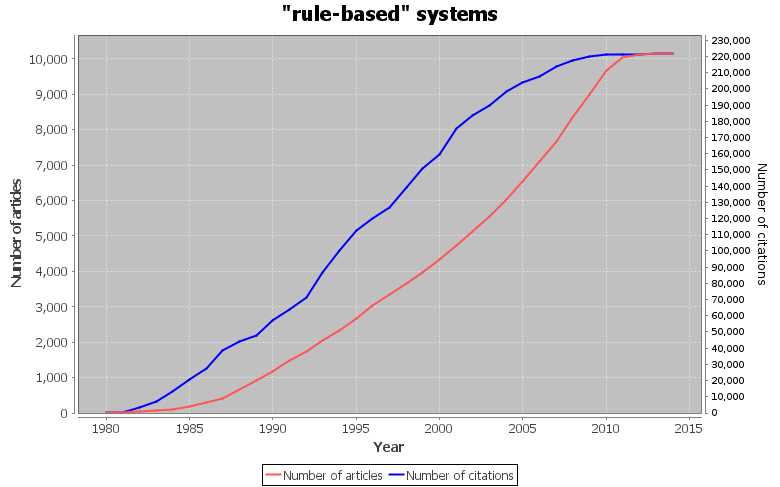
\includegraphics[width=0.95\textwidth]{scholar-rule-based}
	\caption{Google Scholar and Microsoft Academic Search accumulated trending for ``rule-based systems'' query \cite{Rus:scholar-trends}.}
	\label{fig:scholar-rule-based}
\end{figure}

Although the proposed solution is not a rule-based system per se, it uses a simple rule-based component (see more about that in \cref{sec:architecture}).

The \emph{rules} mentioned earlier are most often written in the form of \texttt{IF~a~THEN~b}, where this \texttt{a} and \texttt{b} components may represent almost anything \cite{Smith:krr}. In particular, the \texttt{b} part could be an assertion of some other information (that is adding the new information to the knowledge base). The \emph{facts} are just simple facts.

In very simple terms, an example of a fact could be \texttt{Ann is a human}. If it had also its corresponding rule defined, say, \texttt{IF \underline{X} is a human, THEN \underline{X} is going to die}, it would be possible to infer and assert the fact that \texttt{Ann is going to die}. Similarly, facts can be retracted (or deleted) from the knowledge base.

In thinking about how this approach is different from regular programming--- ``regular'' as in ``imperative'', as functional programming shows some similarities----it is really important to notice, that---in their purest form, in theory---rule-based systems do not impose any order in which rules are going to be executed. At least, that is the suggested mindset when defining rules of a particular RB system.

\todo{parts of rbs}

\todo{knowledge base}

Some other differences---apart from no obvious order of execution---can be also thought of as advantages of this approach. They are listed below.

\begin{itemize}
	\item \todo{advantages}
\end{itemize}

\section{HeaRTDroid}

One example of rule-based systems that might be of particular interest for this project is HeaRTDroid. As the last part of the name suggests, it is meant to be run on mobile devices controlled by the Android system.